\section{Preliminaries, Spherical Geometry, Definitions, and Notation}\label{sec:prelims}

We begin by introducing some necessary observations, definitions, and terminology
which will be of use later.  
 We use $\R^2$ to denote the 
Euclidean plane with its usual metric;
similarly, $\R^3$ denotes Euclidean 3-space.  We use $\mbb{S}^2$ to denote the \textit{unit 2-sphere}, which can be 
thought of as the set of points in $\R^3$ at Euclidean distance one from the origin.  

\zs{i think saying something like this is important but the way i've written it here it's not really saying anything....}
This surface also has a `usual metric', but it is tricky to write down as a formula.   Intuitively, the distance between two points on the sphere can be found by drawing the \textit{great circle} which passes through these points and then using a circular arc length formula to compute the length of the shorter of the two segments which join the points.  
In this paper, we only consider the sphere and the plane, and leave the consideration of other surfaces, measures, and metrics to future work.










\begin{definition}
	In a metric space, a \textbf{geodesic} between two points is the shortest path connecting them with respect to the metric.
	In the plane, geodesics are line segments, and on the surface of the sphere, geodesics are segments of great circles.
\end{definition}





Geodesics are intricately tied to the metric of the space we're working with, because one way to think of the metric distance between two points is as the length of the shortest geodesic connecting them.  We also note that in the plane, there is a \textit{unique} line segment between any two distinct points, whereas on the sphere, there are two such geodesic segments.  This leads to the definition of a \textit{spherical line}.


\begin{definition}
	On the sphere, the lines are \textit{great circles}, which are the circles of the largest possible radius on the surface of the sphere.  Equivalently, they are the intersections of the surface of the sphere with a plane passing through the center of the sphere.
\end{definition}  

\begin{figure}[htb]
	\centering
	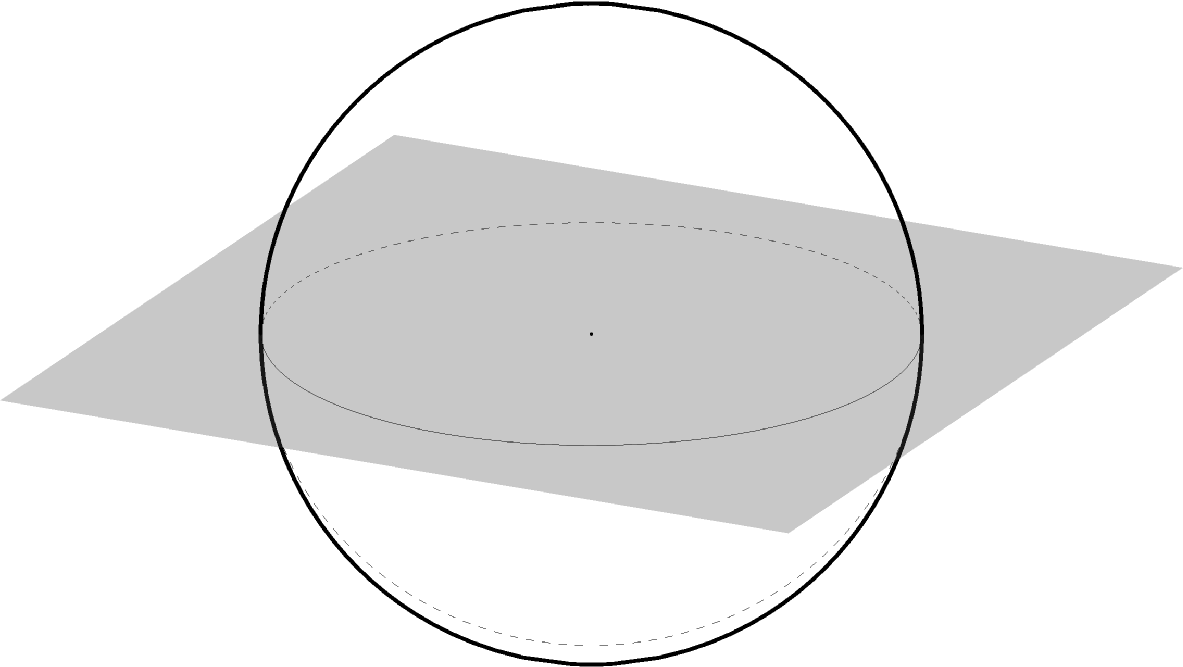
\includegraphics[width=.5\textwidth]{figs/sph-1pl.pdf}
	\caption{A great circle on the sphere with its identifying plane.}
	\label{fig:sphereline}
\end{figure}


In the plane, there is a unique line passing through any two distinct points.  This is almost the case on the sphere, except that we need to exclude one more case.


\begin{observation}
	Given any two points $p$ and $q$ on the sphere which are not antipodal (meaning that our points aren't of the form $p=(x,y,z)$ and $q=(-x,-y,-z)$), there is a unique great circle through $p$ and $q$. 
\end{observation}
\begin{proof}
	To see this, consider the characterization of great circles as the intersections of the surface of the sphere with planes through the center of the sphere.  Since $p$ and $q$ are not antipodes, they are not both collinear with $(0,0,0)$ and so these three points uniquely determine a plane.  This plane intersects the sphere along a great circle which contains $p$ and $q$.
\end{proof}

If $p$ and $q$ \textit{are} antipodal, then any great circle containing one must contain the other as well, so there are infinitely many such great circles.

\begin{figure}[htb]
	\centering
	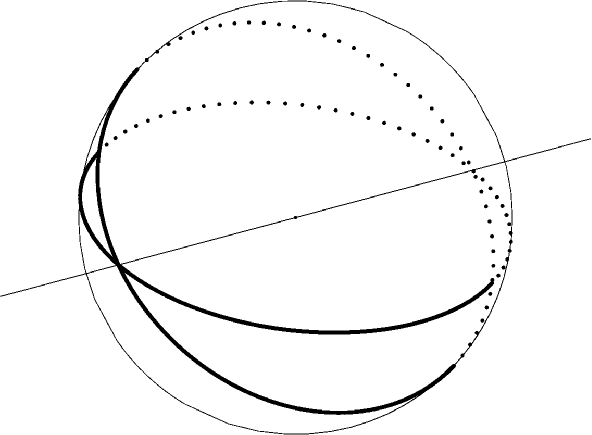
\includegraphics[width=.35\textwidth]{figs/2gc.pdf}
	\caption{Two great circles meet at antipodal points.}
	\label{fig:2gc}
\end{figure}


We now have enough terminology to show a very important fact about spherical geometry.  This  observation is one of the salient features which distinguishes it from the more familiar planar geometry.


\begin{claim}
	Any pair of distinct great circles on the sphere intersect exactly twice, and the points of intersection are antipodes.
\end{claim}
\begin{proof}
	Any two distinct planes determine two distinct great circles, and these planes intersect along a line in $\R^3$ which passes through $(0,0,0)$ and therefore meets the sphere itself at exactly two points, which must be antipodes.
\end{proof}



\zs{the content of this paragraph is important, but the way i've said it is not very clean}
Why is this weird? In the plane, it is always the case that any pair of distinct lines intersects exactly once or they never intersect, in which case we call them \textit{parallel}. Since distinct great circles on the sphere intersect exactly twice, there is no such thing as `parallel lines' on the sphere, and we have to be careful about discussing `the' intersection of two great circles since they do not meet at a unique point.  Furthermore, it is not the case that there is a unique segment of a great circle connecting any two points; there are two, but unless these two points are antipodes, one of the two segments will be shorter.  This shorter segment is the geodesic connecting those points.



We will use this distinction to derive a result which we will use critically in the main theorems of this paper, namely\\

\noindent\textbf{\Cref{lem:sphtri}.}
\emph{The sum of the interior angles of a spherical triangle is strictly greater than $\pi$.  More specifically, the sum of the interior angles is equal to $\pi$ plus the area of the triangle.}

Contrast this to the planar setting, where the sum of the interior angles of a triangle is equal to $\pi$ for any triangle, regardless of its area.  As a concrete example, we can construct a spherical triangle with three right angles.  The triangle formed by the north pole and two points on the equator, one a quarter of the way around the sphere from the other, form such a triangle.  Its area is one eighth of the whole sphere, or $\tfrac{\pi}{2}$, which is, not coincidentally, equal to $\tfrac{\pi}{2}+\tfrac{\pi}{2}+\tfrac{\pi}{2} - \pi$.


In order to  show \Cref{lem:sphtri}, we need some way to translate between \textit{angles} and \textit{area}.  To do that, we'll use a shape which doesn't even exist in the plane: the \textit{diangle} or \textit{lune}.  Consider two distinct great circles.  We know they intersect at two antipodal points, and we can also see that they cut the surface of the sphere into four regions.  Consider one of these regions.  Its boundary is a pair of great circle segments which connect antipodal points and meet at some angle $\theta$ at both of these points.  This shape is a polygon with two sides, hence the name `diangle'.  The term `lune' refers to the crescent moon-shape of this kind of region, and is the term we will use going forward.  \mute{On the Earth, a lune is the region between any two lines of longitude, for example.}

The area of a lune with angle $\theta$ is easy to compute.


\begin{figure}[htb]
	\centering
	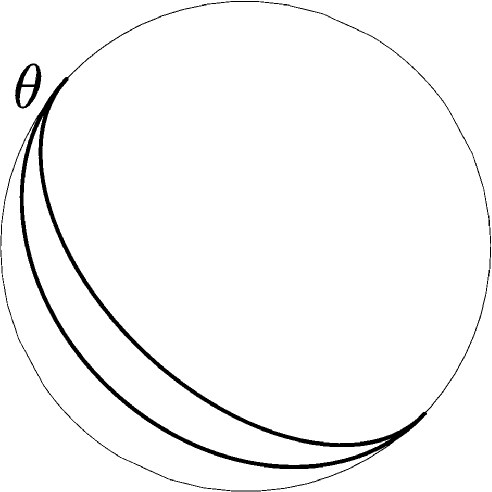
\includegraphics[width=.35\textwidth]{figs/lune.pdf}
	\caption{A lune corresponding to an angle $\theta$. }
	\label{fig:lune}
\end{figure}

\begin{claim}
	Consider a lune whose boundary segments meet at angle $\theta$.  Then the area of this lune is $2\theta$.
\end{claim}
\begin{proof}
	This claim follows from observing that a lune with angle $\theta$ occupies a $\tfrac{2\pi}{\theta}$ portion of the sphere's surface area.  The total surface area of the sphere is $4\pi$, so a lune with angle $\theta$ has surface area $\tfrac{4\pi\theta}{2\pi}= 2\theta$.
\end{proof}

Now that we have a tool that lets us relate angles and areas, we can finally prove the main result of this section.










\begin{lemma}\label{lem:sphtri}
	
	The sum of the interior angles of a spherical triangle is strictly greater than $\pi$.  More specifically, the sum of the interior angles is equal to $\pi$ plus the area of the triangle.
\end{lemma}

\begin{proof}
	Consider a triangle on the sphere with angles $\theta_1$, $\theta_2$, and $\theta_3$.  Let $T$ denote the area of this triangle. If we extend the sides of the triangle to their entire great circles, each pair intersects at the vertices of our triangle as well as the three points antipodal to the vertices of our triangle, and at the same angles at both sets of points.  This triangle is congruent to our triangle, so its area is also $T$.  Each pair of lines cuts the sphere into four lunes, one which contains our triangle, one which contains the antipodal triangle, and two which do not contain either triangle.  We are interested in the three pairs of lunes which do contain the triangles.  We will label these lunes by their angles, so we have a lune $L(\theta_1)$ and its antipodal lune $L'(\theta_1)$, and we can similarly define $L(\theta_2)$, $L'(\theta_2)$, $L(\theta_3)$, and $L'(\theta_3)$.
	
	
	\begin{figure}[htb]
		\centering
		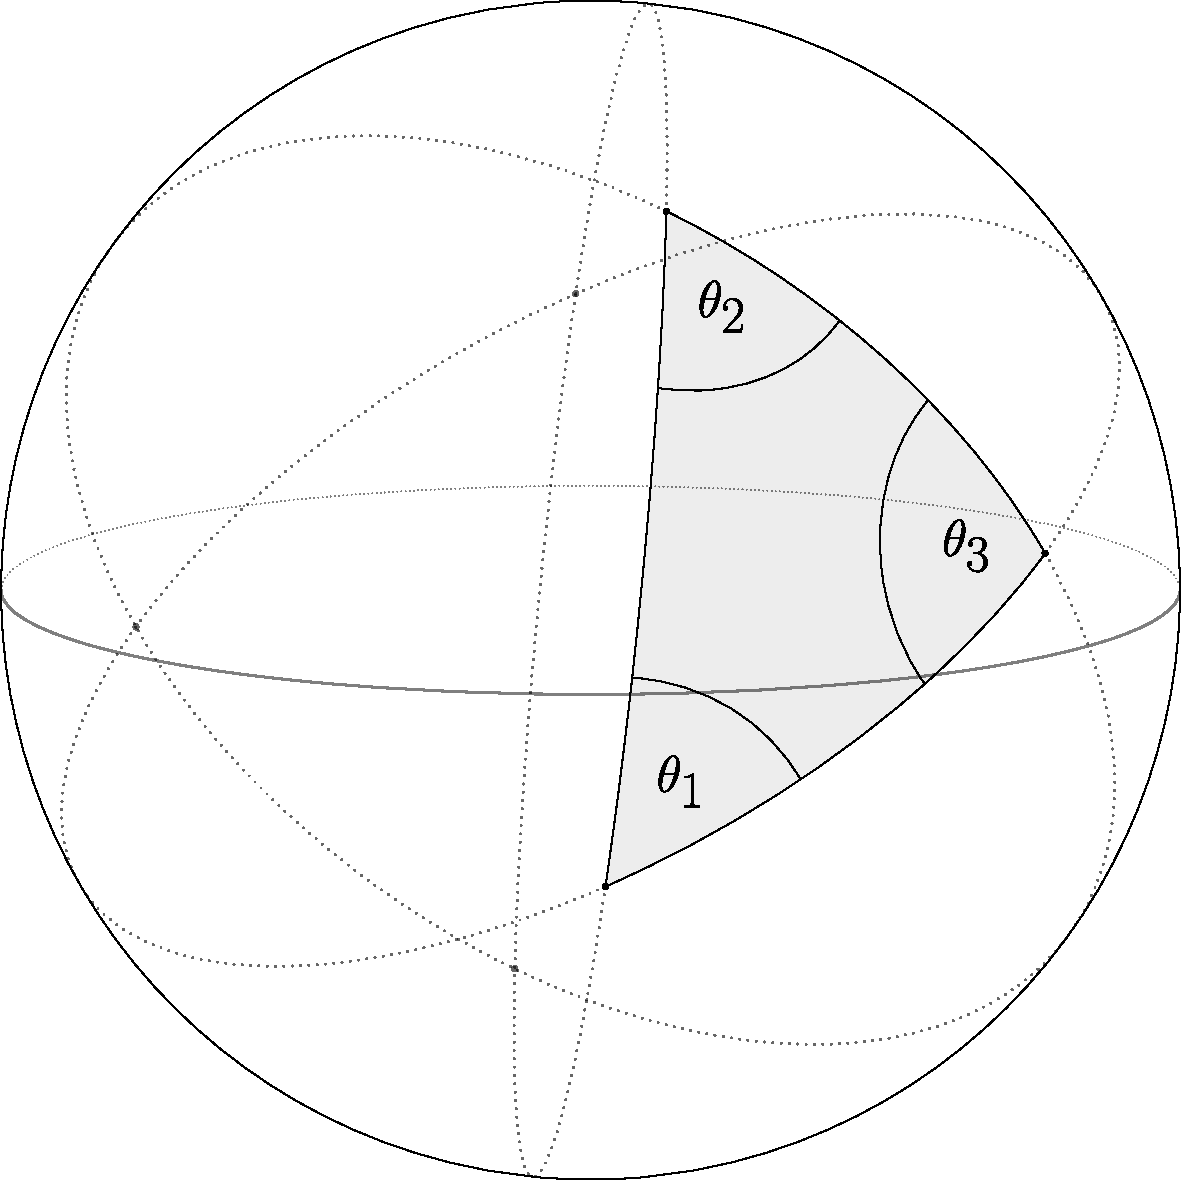
\includegraphics[width=.35\textwidth]{figs/trilune.pdf}
		\caption{A spherical triangle and the antipodal triangle define six lunes.}
		\label{fig:trilune}
	\end{figure}
	
	
	We have six lunes.  In total, they cover the sphere, but share some overlap.  If we remove our triangle from two of the three which contain it and the antipodal triangle from two of the three which contain it, then we have six non-overlapping regions which cover the sphere, so the area of the sphere must be equal to the sum of the areas of these six regions.  We can write
	
	\begin{align*}
	4\pi &= \mathrm{area}(L(\theta_1)) + \mathrm{area}(L'(\theta_1)) \\
	&+  (\mathrm{area}(L(\theta_2)) - T) + (\mathrm{area}(L'(\theta_2)) - T) \\
	&+ (\mathrm{area}(L(\theta_3)) - T)	 + (\mathrm{area}(L'(\theta_3)) - T).
	\end{align*}
	
	And by the earlier claim, we know that the areas of the lunes are twice their angles, so we can rewrite this as
	
	
	\begin{align*}
	4\pi &= 2\theta_1 + 2\theta_1 
	+  (2\theta_2 - T) + (2\theta_2-T) 
	+ (2\theta_3 - T)	 + (2\theta_3 - T)
	\end{align*}
	
	which simplifies to 
	
	\begin{align*}
	\theta_1+\theta_2+\theta_3 = \pi + T,
	\end{align*}
	
	which is exactly the statement we wanted to show.
\end{proof}

We will need one more fact about spherical triangles before we conclude this section.  It dates back to (at least) Euclid's \textit{Elements} \cite{elements} where it follows from Propositions I.6 and I.8.  

\begin{claim}
	An equilateral triangle is equiangular, and vice versa.
\end{claim}

While \textit{Elements} is a compendium of facts about planar geometry, these two propositions do not rely on the assumption that parallel lines exist, and so they hold on the surface of the sphere as well.  
\begin{proof}
	To show them, first suppose that we have a triangle with vertices $a$, $b$, and $c$ and suppose that the length of the side $ab$ is equal to that of $bc$, and let $m$ be the midpoint of the segment $bc$.  Consider the segment $am$. This splits the triangle $abc$ into two triangles $amb$ and $amc$ which have equal side lengths and are therefore congruent.  By this congruence, the angle opposite $a$ is equal to the angle opposite $c$.
	
	To see the converse, suppose that the angles opposite $a$ and $c$ are equal.  Then the triangles $abc$ and $acb$ are congruent, since \Cref{lem:sphtri} implies that if there are two triangles with the same angles, then their areas are equal as well and they are therefore congruent.
\end{proof}


Now that we have built the necessary tools of spherical geometry, we will wrap up this section with a battery of definitions. 
We carefully lay out these definitions so
as to align with an intuitive understanding of the concepts and to
appease the astute reader who may be concerned with edge cases,
geometric weirdness, and nonmeasurability. 









\begin{definition}
	A \textbf{region} $\Omega$ in $\mathbb{S}^2$ or 
	in $\R^2$ is a non-empty open set together with its
	boundary, such that $\Omega$ is compact and the boundary can be described piecewise as 
	a finite collection of smooth curves.
\end{definition}

This definition is highly technical to allow us to assume away any annoying edge 
cases that might crop up.  Piece-by-piece, a \textit{non-empty open set} lets us 
talk about the \textit{area} of a region in a sensible way. Specifying that a region 
must be \textit{compact} gets rid of cases where we have to worry about regions having 
infinite area.  The entire plane should not be considered a `region'.  Finally, the 
\textit{piecewise-smooth boundary} condition gives us a way to talk about the \textit{perimeter} 
of a region.  We don't want to have to worry about fractal-like shapes which have well-defined 
area but an infinite perimeter or shapes such as a collection of line segments which meet at a point, which has a well-defined perimeter but no area.










\begin{definition}
  A \textbf{compactness score function} $\mathcal{C}$ is a function from
  the set of all regions to the positive real numbers.  We adopt the
  convention that a region with a \textit{higher} compactness score is
  \textit{more} compact, and this naturally induces a partial order over
  the set of all regions, where $A$ is at least as compact as $B$ if and
  only if $\mathcal{C}(A)\geq \mathcal{C}(B)$.
\end{definition}

The final major definition we need is that of a \textit{map
projection}.  In reality, the regions we are interested in comparing
sit on the surface of the Earth (i.e. a sphere), but these regions are
often examined after being projected onto a flat sheet of paper or
computer screen, and so have been subject to such a projection.

\begin{definition}
  A \textbf{map projection} $\varphi$ is a 
  diffeomorphism from a region on the sphere to a region on the 
  plane. 
\end{definition}

Intuitively, a map projection is a well-defined, invertible function between the sphere and the plane which sends regions on the sphere to regions in the plane.  Throughout, we use $\vphi$ to denote such a function from a region of the sphere 
to a region of the plane and $\vphi^{-1}$ its inverse, which goes from a region of the plane to a region of the sphere. 

\begin{definition}
  We use the word \textbf{transformation} [of the plane/sphere] to mean
  to a diffeomorphism from the plane or sphere to itself.
\end{definition}

Since the image of a region under a map projection $\varphi$ is also
a region, we can examine the compactness score of that region both 
before and after applying $\varphi$, and this is the heart of the
problem we address in this paper.  We demonstrate, for several
examples of compactness scores $\mathcal{C}$, that the order
induced by $\mathcal{C}$ is different than the order induced by
$\mathcal{C}\circ\varphi$ for \textit{any} choice of map projection
$\varphi$.

\begin{definition}
  We say that a map projection $\vphi$ \textbf{preserves the  
  compactness score ordering} of a score $\mc{C}$ if for any regions 
  $\Omega,\Omega'$ in the sphere, $\mc{C}(\Omega)\ge \mc{C}(\Omega')$ 
  if and only if $\mc{C}(\vphi(\Omega)) \ge \mc{C}(\vphi(\Omega'))$ in the plane.
\end{definition}

   This is a weaker condition than simply preserving the raw compactness scores. 
   If there is some map projection which results in adding $.1$ to the score of each region, the raw scores are certainly not preserved, but the ordering of regions by their scores is. Additionally, $\vphi$ preserves a compactness score ordering 
  if and only if $\vphi^{-1}$ does.


\zs{this should be moved to the geometry section}
\begin{definition}
  A 
  \textbf{cap} on the sphere  $\mbb{S}^2$ is a region on the sphere
 which can be described as all of the points on the sphere to one side of some plane 
 in $\R^3$.  A cap has a \textit{height}, which is the largest distance between this cutting plane and the cap, and a \textit{radius}, which is the radius of the circle formed by the intersection of the plane and the sphere.  See \Cref{fig:caphr} for an illustration.
\end{definition}


\begin{figure}[h]
  \centering
  %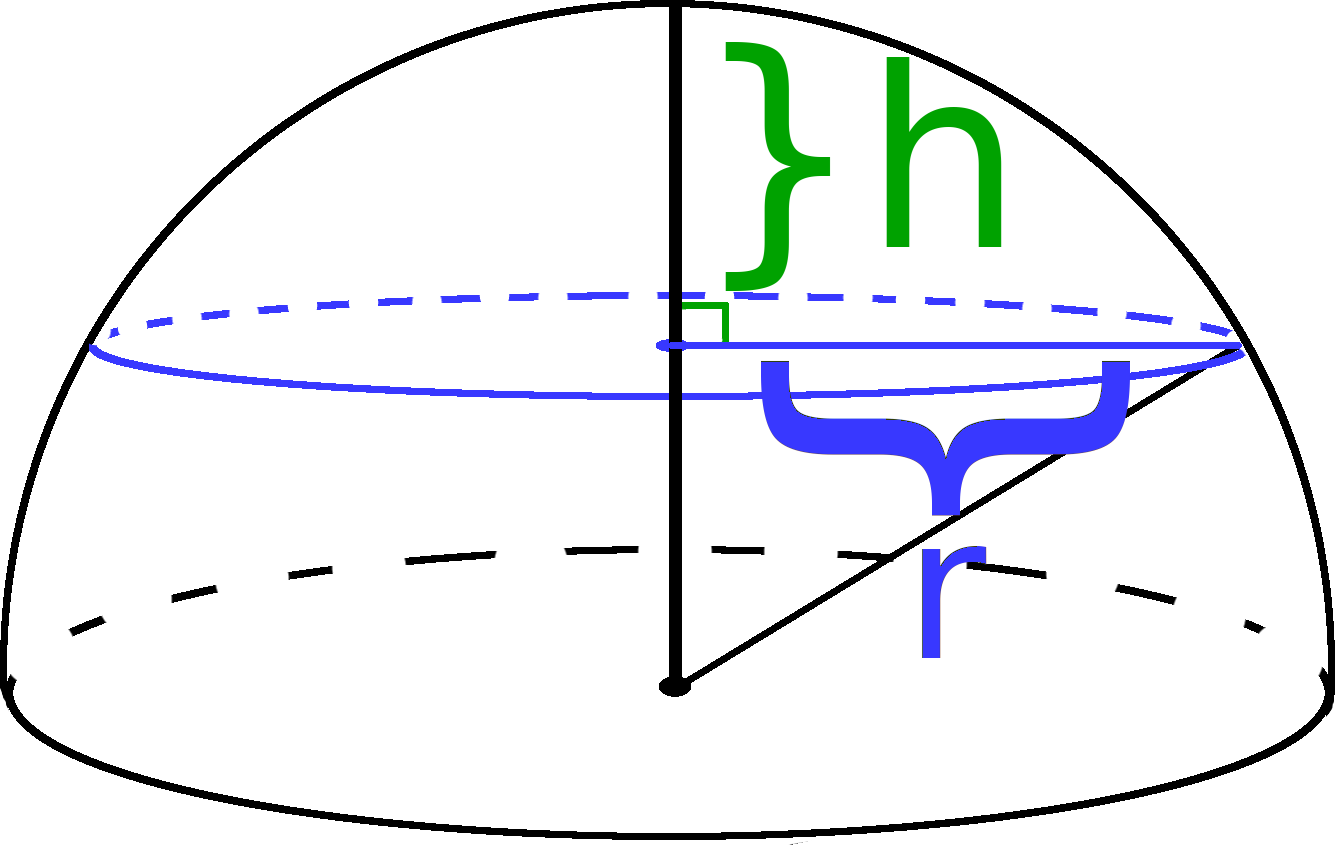
\includegraphics[width=.3\textwidth]{figs/spherecapschema}\\[1.5em]
  \definecolor{qqqqff}{rgb}{0,0,1}

\definecolor{ccqqqq}{rgb}{0.8,0,0}

\definecolor{ududff}{rgb}{0.30196078431372547,0.30196078431372547,1}

\begin{tikzpicture}[line cap=round,line join=round,>=triangle 45,x=1cm,y=1cm]

\clip(-4.493355050909743,-1.2748355780287404) rectangle (4.462150807191927,4.785872976331056);

\draw [shift={(0,0)},line width=3.2pt]  plot[domain=0:3.141592653589793,variable=\t]({1*4*cos(\t r)+0*4*sin(\t r)},{0*4*cos(\t r)+1*4*sin(\t r)});

\draw [shift={(0.0016366799970421299,9.441278259356354)},line width=2pt]  plot[domain=4.286394541961201:5.138764290071874,variable=\t]({1*7.708897306730456*cos(\t r)+0*7.708897306730456*sin(\t r)},{0*7.708897306730456*cos(\t r)+1*7.708897306730456*sin(\t r)});

\draw [shift={(0.019848790872865698,-6.481795867514522)},line width=2pt,dotted]  plot[domain=1.22830273729039:1.9174384984929125,variable=\t]({1*9.441973016351305*cos(\t r)+0*9.441973016351305*sin(\t r)},{0*9.441973016351305*cos(\t r)+1*9.441973016351305*sin(\t r)});

\draw [line width=2pt,color=ccqqqq] (0,2.4033620491027756)-- (0,4);

\draw [line width=2pt,color=qqqqff] (0,2.4033620491027756)-- (3.2001911763834157,2.3997450770024993);

\begin{scriptsize}

\draw [fill=ududff] (0.0016366799970421299,9.441278259356354) circle (2.5pt);

\draw [fill=ududff] (0.019848790872865698,-6.481795867514522) circle (2.5pt);

\draw[color=ccqqqq] (0.26805571312169243,3.3034918797019284) node {\LARGE$h$};

\draw[color=qqqqff] (1.6285727817769453,2.167711482419824) node {\LARGE $r$};

\end{scriptsize}

\end{tikzpicture}
  \caption{ The height $h$ and radius $r$ of a spherical cap. }
  \label{fig:caphr}
\end{figure}





